\documentclass[12pt, a4paper]{IEEEtran}

\usepackage{amsmath,amssymb,amsfonts}
\usepackage{graphicx}
\usepackage{textcomp}
\usepackage{xcolor}
\usepackage{blindtext}
\usepackage{dirtytalk}
\usepackage{caption}
% \usepackage{listings}
% \usepackage{minted}
% \definecolor{DarkGray}{gray}{0.1}
% \usemintedstyle{pastie}
    
\begin{document}

\title{Music Identification through Audio Fingerprinting}

\author{
    \vspace{10mm}
    \huge
    Group 1 \\
    \vspace{3mm}
    \LARGE
    Yashraj Kakkad - \textit{AU1841036} \\ 
    Prayag Savsani - \textit{AU1841035} \\
    Yashil Depani - \textit{AU1841005} \\ 
    Harshil Mehta - \textit{AU1841010} \\
\vspace{3mm}
Guided by - Prof. Ashok Ranade \\
\null \vfill
*The photo goes here*
}

\begin{titlepage}
    \begin{center}
        \vspace*{1cm}
        
        \Huge
        \textbf{Music Identification through Audio Fingerprinting}
        
        \vspace{1cm}
        \LARGE
        Group 1 \\
        \vspace*{3mm}
        Yashraj Kakkad - \textit{AU1841036} \\ 
        Prayag Savsani - \textit{AU1841035} \\
        Yashil Depani - \textit{AU1841005} \\ 
        Harshil Mehta - \textit{AU1841010} \\
        
        \vspace*{3mm}
        Guided by - Prof. Ashok Ranade

        \vspace*{5cm}
        *The group photo goes here*

    \end{center}
\end{titlepage}

\section{Objective}
The objective of the project is to recognize a song from an arbitrary 30 second sample through appropriate audio fingerprinting techniques.
To accomplish that, a number of songs are broken into chunks. The best frequencies across a spectrum are taken and they are hashed in an appropriate data structure.
The obtained input from the user undergoes a similar procedure and is then compared with the hash values of the song. The song which matches with the input the most is displayed as a result to the user.
\par
This was a very brief outline. The coming sections exactly explain what we have done.
\begin{figure}[h]
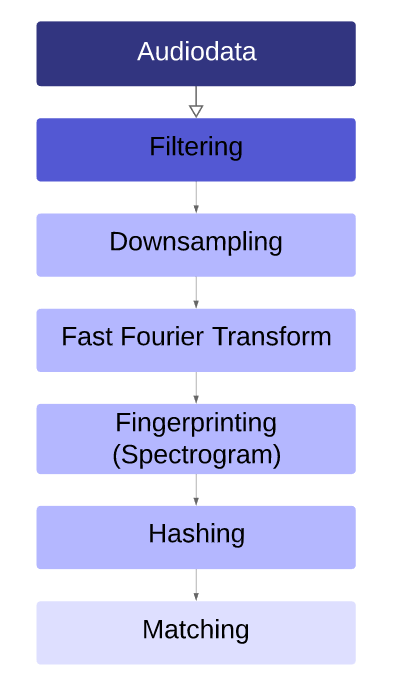
\includegraphics{Flowchart.PNG}
\captionsetup{justification=centering}
\caption{Flowchart explaining our fingerprinting algorithm in brief}
\end{figure}
\section{Sampling}
Music is typically sampled at 44.1 kHz. This is because of a theorem by Nyquist and Shannon which requires \(f_d >= 2f_s\) where \(f_d\) is the digital frequency and \(f_s\) is the sampling rate. The number, in practice, is greater than 2. Maximum sound frequency, as we know, is 20 kHz.
\par
We'll be using Fast Fourier Transform at a later stage to obtain the frequency spectrum of several chunks of the song. Running it on even a few hundred songs would take days.
Therefore, we downsample the recorded sample by a factor of 4. 
As a consequence, the maximum sound frequency in our audio sample comes down to 5kHz. This is not a problem as the frequency spectrum of most of the song lies below 5kHz. The gains are therefore much higher than the losses.

\section{Filtering}
Aliasing refers to the distortion that results when a signal reconstructed from samples is different from the original continuous signal.
We filter the high-end frequences before downsampling to avoid this phenomenon. We use a 5th order butterworth low-pass filter to achieve the same.
\begin{figure}[h]
    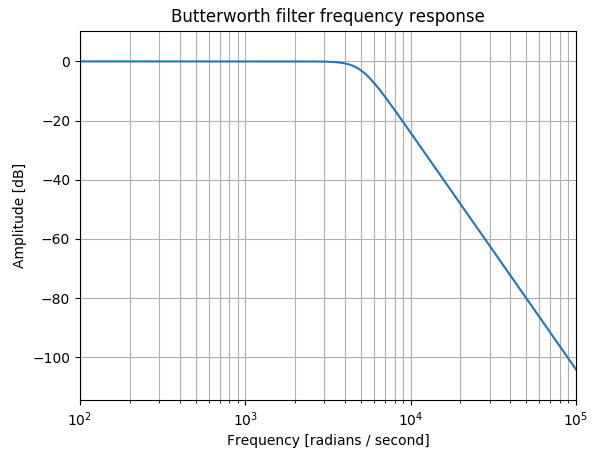
\includegraphics[width=0.5\textwidth]{lowpassfilter.png}
    \captionsetup{justification=centering}
    \caption{Frequency response of a butterworth low-pass filter from Sci-py package in Python}
\end{figure}
\section{Fast Fourier Transform}
Discrete Fourier Transform converts a signal from the time domain to the frequency domain. The formula is:
\begin{align*}
    X(n) = \sum_{k=0}^{N-1} x[k] e^{-j(2\pi kn/N)}
\end{align*}
Here,
\begin{itemize}
    \item N is the window size
    \item X(n) is the \(\text{n}^{th}\) bin of frequencies
    \item x(k) is the \(\text{k}^{th}\) sample of audio signal
\end{itemize}
\par
Fast Fourier Transform is an algorithm that computes Discrete Fourier Transform. As the name says, it is "faster" than actual Discrete Fourier Transform. To make a comparison, Discrete Fourier Transform requires \(\mathcal{O}(N^2)\) while its counterpart only requires \(\mathcal{O}(NlogN)\), where N is the number of samples. This is a huge improvement since N is typically quite large in our case.
\par
Speed is important in this case as the quicker we get the answer, the better experience we provide to the user.
Also, the database of songs to be maintained is large.

\section{Windowing}
We cannot directly perform Fast Fourier Transform on the whole song. A typical song has many frequencies and the input from the user can be any part of the song containing any of these frequencies. 
\par
We therefore intend to apply Fast Fourier Transform on small chunks successively. For doing so, we need to extract the appropriate parts of the song. 
We do that by multiplying our audio signal with an appropriate window function. But by \say{multiplying}, we are introducing new frequencies that did not exist before in the audio signal. This is known as spectral leakage. 
\par
Window size is 4096 samples. That makes our spectral resolution to be 0.37 seconds, effectively meaning that the algorithm can detect changes in the song for every 0.37 seconds.
\par
We cannot avoid spectral leakage in this case but we can handle its behavior by appropriately choosing our window function.
Some window functions, like the \say{usual} rectangular window function, lead to spectral leakage. Others, like Blackman are particularly bad with noise.
We choose Hamming Window for our purpose since its performance lies between the two extrema.
\begin{figure}[h]
    \centering
    \includegraphics[width=0.45\textwidth]{hamming.png}
    \captionsetup{justification=centering}
    \caption{Hamming Window Function}
\end{figure}
\vspace*{16mm}
\section{Fingerprinting}
An audio fingerprint can be considered a digital summary which helps to identify an audio sample from a given audio database. Audio fingerprints differ from standard computer fingerprints like SSHA or MD5 because two different files containing the same music must possess the same audio fingerprint which wouldn't be the case with their SSHA or MD5 fingerprints. This is why, audio fingerprints are generated using filtered spectrograms of audio samples which only contain data regarding the frequencies present in the song.

\subsection{Spectrogram}
A three dimensional graph where
\begin{itemize}
    \item X-axis indicates time
    \item Y-axis indicates frequency
    \item Color indicates amplitude of a frequency at a given time 
\end{itemize}
\begin{figure}[h]
\begin{center}
    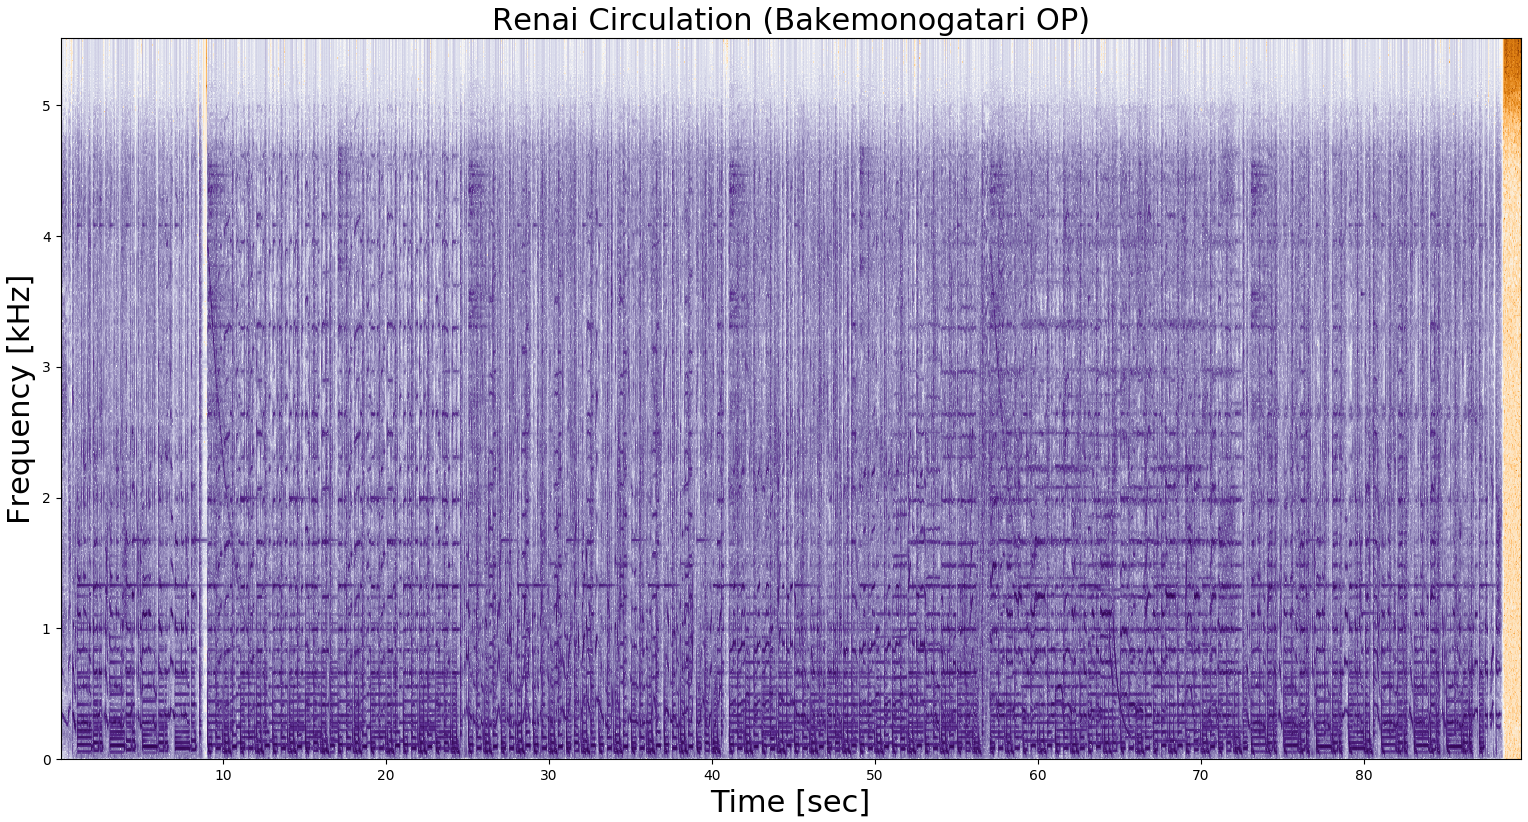
\includegraphics[width=0.5\textwidth, height=0.2\textwidth, keepaspectratio]{ActualSong.png}
\end{center}
\captionsetup{justification=centering}
\caption{Spectrogram of a full length song}
\end{figure}
\begin{figure}[h]
    \begin{center}
        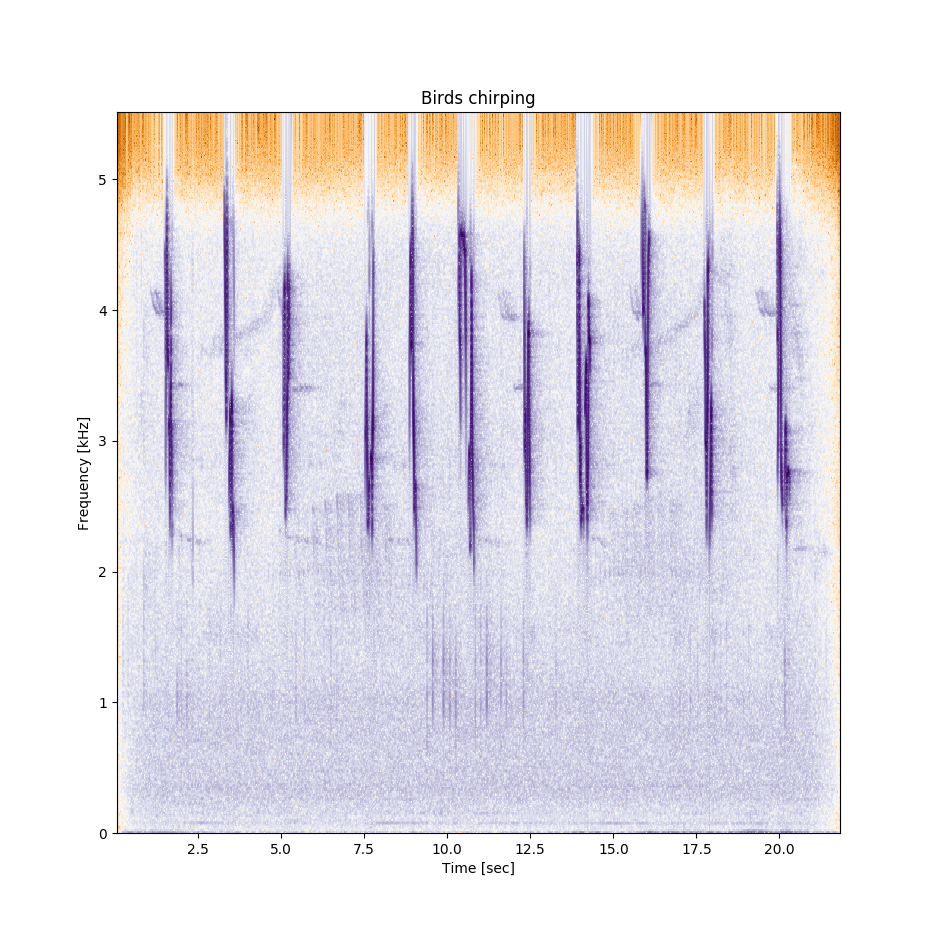
\includegraphics[width=0.5\textwidth, height=0.4\textwidth, keepaspectratio]{BirdsChirping.png}
    \end{center}
    \captionsetup{justification=centering}
    \caption{Spectrogram of a song with sharp peaks}
    \end{figure}
Using the frequencies obtained from FFT, a spectrogram can be generated. For a filtered spectrogram, you need to extract the minimum number of frequencies that you need to uniquely identify a given audio sample.

\subsection{Filtering the ocean of frequencies}

While looking for the most important frequencies, we are looking for frequencies with the strongest amplitudes which are also called peaks. This is done because the algorithm needs to be as noise tolerant as possible. As different songs will have these frequencies in different frequency ranges, we divide our whole frequency spectrum (0-5 kHz) into 5 frequency ranges. They are -
\begin{itemize}
    \item 30-40 Hz
    \item 40-80 Hz
    \item 80-120 Hz
    \item 120-180 Hz
    \item 180-600 Hz
\end{itemize}
Using this frequency data, we can now a plot the filtered spectrogram of the audio sample which looks like this -
This filtered data effectively acts as our audio fingerprint and can now be hashed to decrease processing times.

\section{Hashing}
Hashing is an efficient way to store these values as comparing hash values is an \(\mathcal{O}(1)\) operation.
Now that we have the most relevant frequencies across five bins for every window, they can be hashed into a single number and stored in the database. The hashing formula involves a factor for error correction conveniently called 'fuzzy' factor. This is there because recording conditions are not always perfect and there needs to be a variable factor to adjust these hash values.
We use the following algorithm to hash our values:
HASHING ALGORITHM GOES HERE

\section{Matching}
This is perhaps the most important part of the process.
We perform the exact same operations on our recorded sample from the user.
Should just matching the hash values help us identify which song it is? Maybe yes, but there's a more effective algorithm to accomplish the same.
\par
Besides the hash values, we also have the relative time in which they're present in the song as the stored values are sequential.
If:
\begin{itemize}
    \item sample \#1 of our recording matches with sample \#25 of a particular song
    \item sample \#3 matches with sample \#28 and
    \item sample \#8 matches with sample \#32,   
\end{itemize}
we can safely claim that the song recorded is the song we're talking about.
This is because the relative offset in these cases is the same: \(24 = 25 - 1 = 28 - 3 = 32 - 8\). \\
\begin{figure}[h]
    \begin{center}
        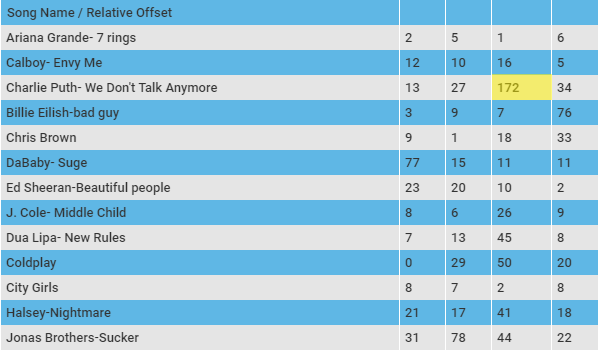
\includegraphics[width=0.5\textwidth]{matching.png}    
    \end{center}
    \captionsetup{justification=centering}
    \caption{Illustration of the result of our matching algorithm. The song corresponding to the maximum offset is our answer.}
\end{figure}
\par
We can summarize our matching process as under:

\begin{itemize}
    \item Record a sample and perform the above steps on the recorded sample.
    \item Load the database of hash values
    \item For every hash value, identify the songs having that hash value. Keep track of the relative offset.
    \item Return the song (or few best songs) having a hash value with the maximum number of offsets across all songs and all hash values.
\end{itemize}

\section{Results}
We tested the algorithm in several situations and here are the conclusions:
We took random 30-second cuttings of the songs and put them to test. The success rate was 100\%. The algorithm didn't fail even once.
\par
However, in real world situations, several factors come to play. The quality of speakers as well as the microphone matters and there's some noise too.
With a decent phone microphone and minimal noise, the accuracy is reasonably good.
\par
Here's a comparison of the spectrograms of the same song and the same duration. The first one is a recording and the second one is cut from the song. As it can be seen, they are reasonably similar. 
\vspace{-5mm}
\begin{figure}[h]
    \begin{center}
        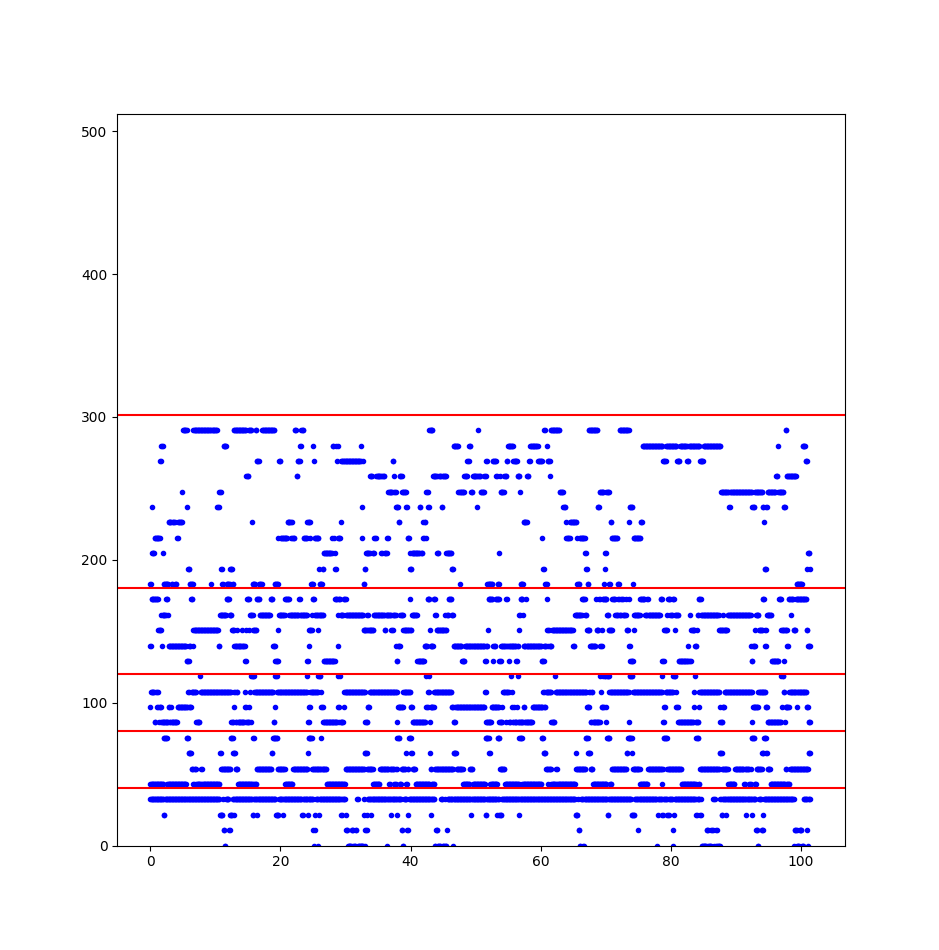
\includegraphics[width=0.475\textwidth]{Plot_CT.png}
    \end{center}
    \captionsetup{justification=centering}
    \caption{Spectrogram of an \textit{extracted} 10 second sample }
\end{figure}
\vspace{-10mm}
\begin{figure}[h]
    \begin{center}
        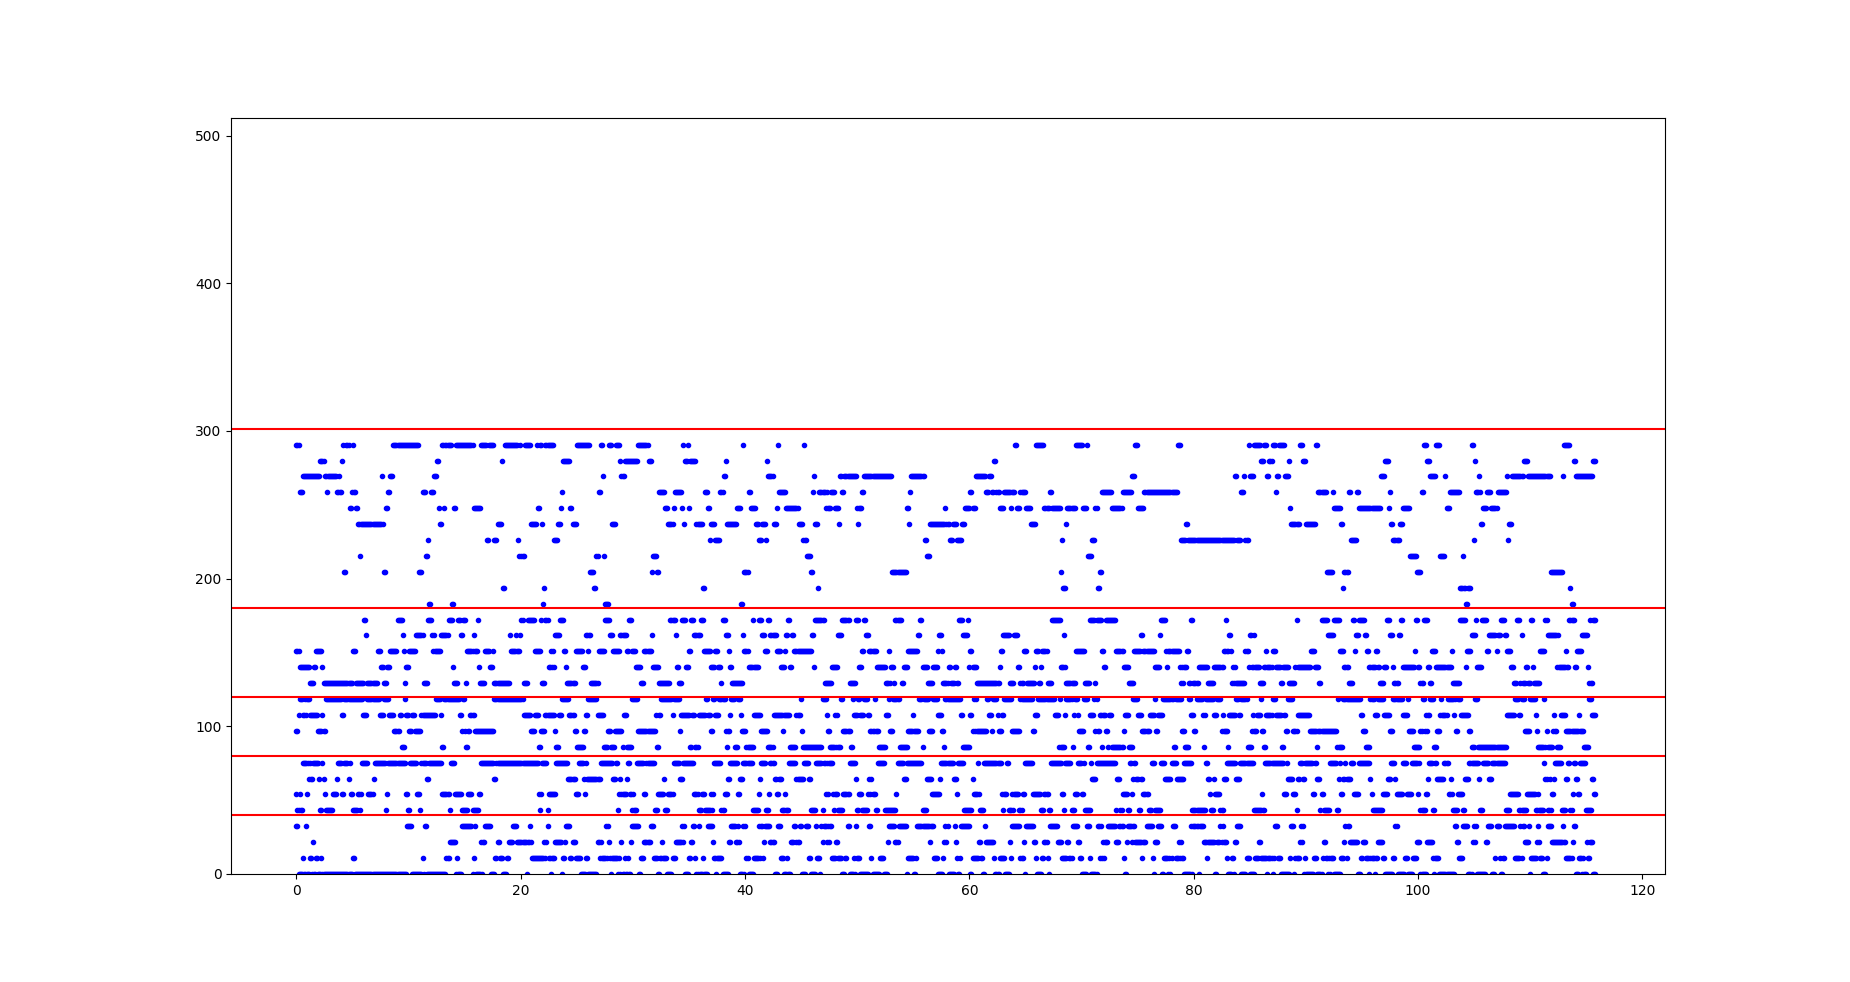
\includegraphics[width=0.475\textwidth, height=0.475\textwidth]{Cheap_Thrills.png}
    \end{center}
    \captionsetup{justification=centering}
    \caption{Spectrogram of a \textit{recorded} 10 second sample }
\end{figure}
\par
We also tinkered other constants in our algorithm, like the samples per window, and settled with 4096 samples. We also took chunks of relative offsets by dividing them by a factor like 5 or 10, but that did not help much at the end.
% \section{Section Title}
% \blindtext

\pagebreak

\onecolumn
\inputminted{python}{song.py}

% \begin{listing}[ht]
% \begin{minted}[
% frame=lines,
% framesep=2mm,
% breaklines=true
% ]{python}
% import numpy as np
    
% def incmatrix(genl1,genl2):
%     m = len(genl1)
%     n = len(genl2)
%     M = None #to become the incidence matrix asdasdfasdfsadfsdfsdafsadfsdfasdsfsdafsdfsadfsadfsdafsdfsadfsadfdsfsdafsadfsadfsadfsadfsdafsdafsadfsadfsadfsadfasdfsadfasdfasdfsadfsadfasdfsadfasdfsdafasdfsadfsadfsdafsadf
%     VT = np.zeros((n*m,1), int)  #dummy variable
    
%     #compute the bitwise xor matrix
%     M1 = bitxormatrix(genl1)
%     M2 = np.triu(bitxormatrix(genl2),1) 

%     for i in range(m-1):
%         for j in range(i+1, m):
%             [r,c] = np.where(M2 == M1[i,j])
%             for k in range(len(r)):
%                 VT[(i)*n + r[k]] = 1;
%                 VT[(i)*n + c[k]] = 1;
%                 VT[(j)*n + r[k]] = 1;
%                 VT[(j)*n + c[k]] = 1;
                
%                 if M is None:
%                     M = np.copy(VT)
%                 else:
%                     M = np.concatenate((M, VT), 1)
                
%                 VT = np.zeros((n*m,1), int)
    
%     return M
% \end{minted}
% \caption{Minimal working example}
% \end{listing}

% \twocolumn
% \section{Section Title}
% \blindtext

\end{document}